% Sidebar subcategory icon: Remeshing (MMG) — the triangulated cavity (the
% "ball" of elements around a node) that a remesher tears down and rebuilds.
% Distinct from `remesh`, the coarse→fine triangle pair used by the Remesh form
% itself. No centre node: at the 14px a .sb-subsection-header renders this at,
% a filled centre merges with the six converging spokes into one blob.
% NOTE: the committed svg-ui/catRemeshing.svg was hand-authored to the same
% drawing (no pdftocairo available); regenerating via `make ui` replaces it with
% the pdftocairo rendering of this source — same glyph either way.
\documentclass[tikz,border=2mm]{standalone}
\usetikzlibrary{arrows.meta,calc,shapes.geometric}
\begin{document}
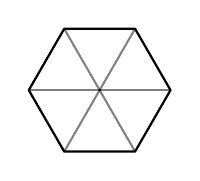
\begin{tikzpicture}[line width=1.3pt, line cap=round, line join=round, x=1mm,y=1mm]
  \foreach \i in {0,...,5} { \coordinate (V\i) at (\i*60:9); }
  \draw[thick] (V0) -- (V1) -- (V2) -- (V3) -- (V4) -- (V5) -- cycle;
  % the spokes are the cavity's elements: lighter, so the hull still reads first
  \foreach \i in {0,...,5} { \draw[line width=0.73pt, opacity=0.5] (0,0) -- (V\i); }
\end{tikzpicture}
\end{document}
